%Nachdem die theoretischen Grundlagen und der Aufbau des ALICE Experiment n\"aher erl\"autert wurden, wird im folgenden die Vorgehensweise erkl\"art, wie $\pi^{0}$ gemessen werden.
%\newline
Die gew\"ahlten \textit{Cluster} nach den Kriterien aus Abschnitt \ref{s3s1s2} bestehen fast ausschlie{\ss}lich aus Photonen oder konvertierten Photonen.
\newline
\begin{figure}[tp]
\centering
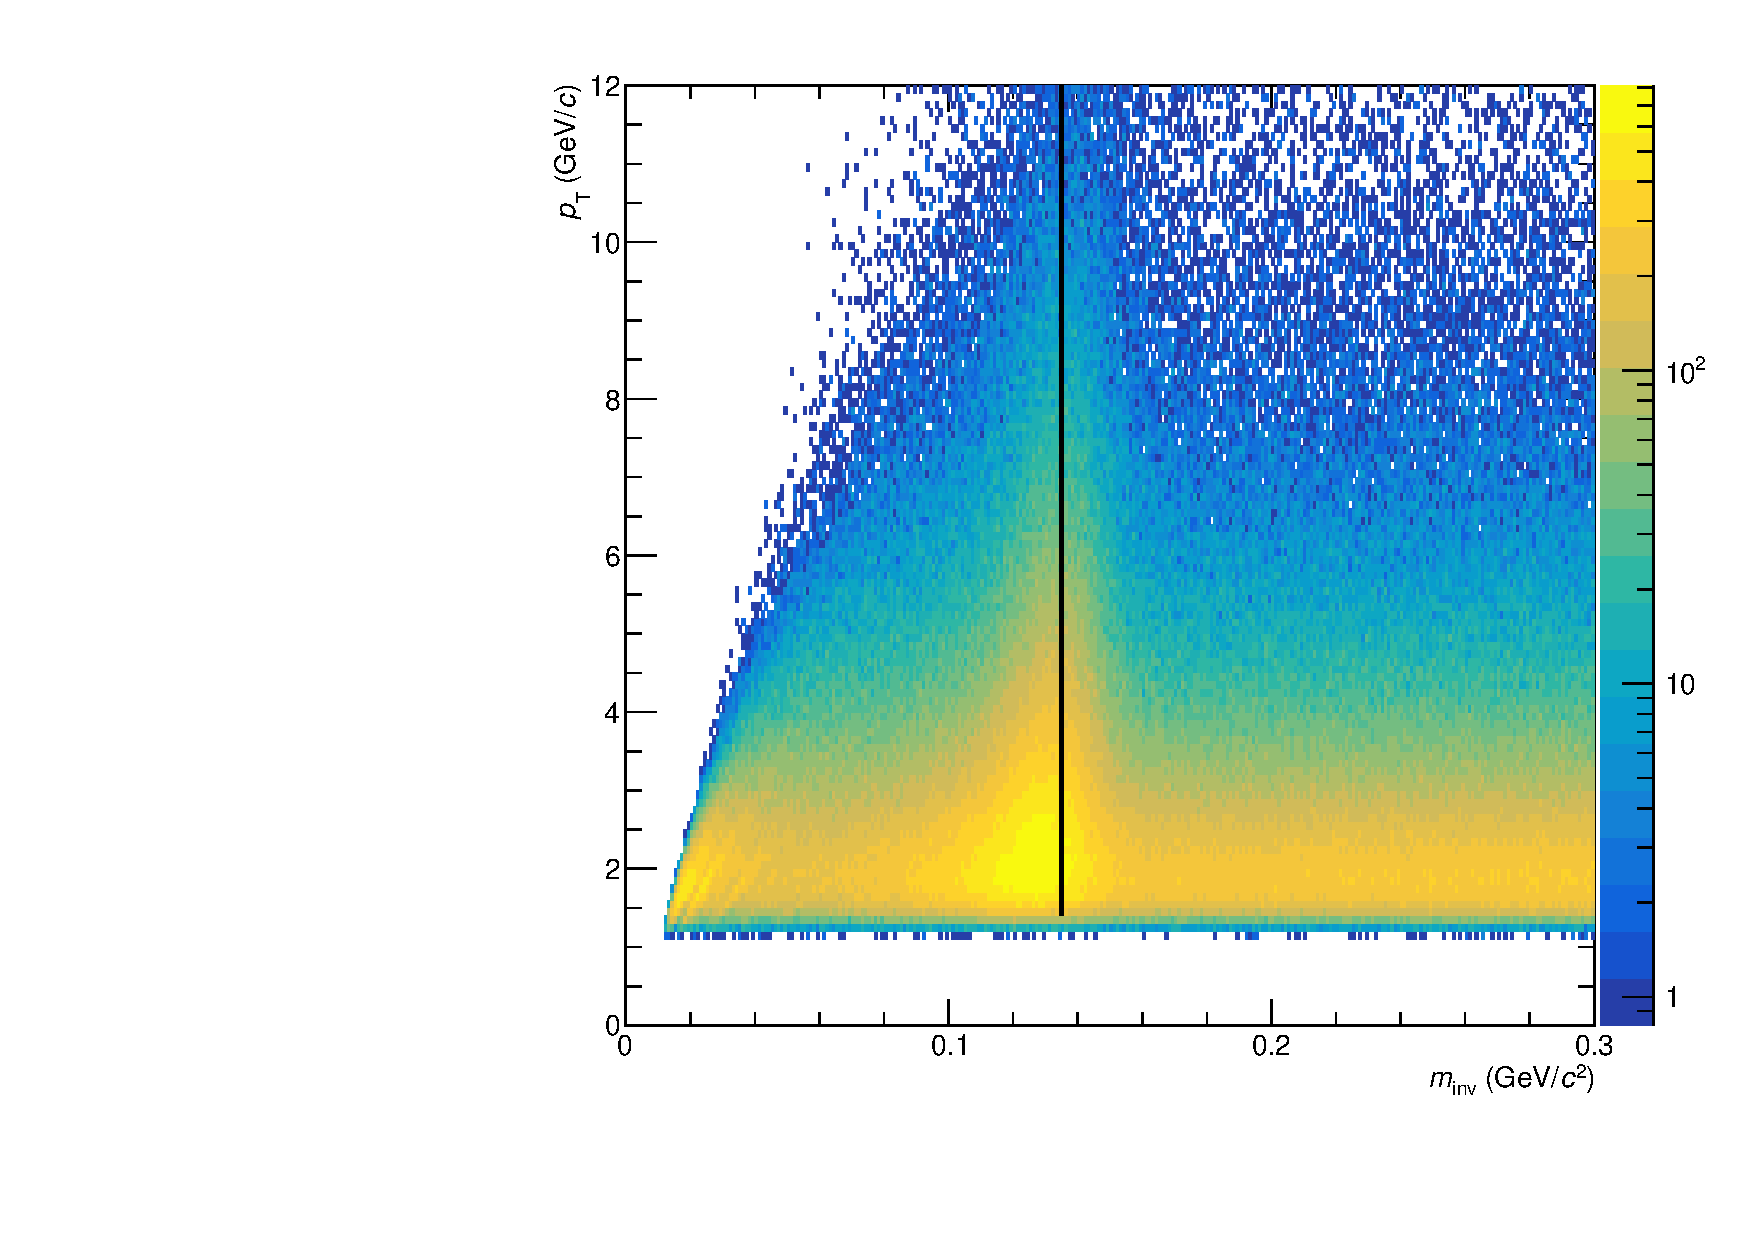
\includegraphics[width=.7\linewidth]{hInvMass_pT_Signal.pdf}
\caption{$p_\text{T}$ und $m_\text{inv}$ als Funktion von der Anzahl von rekombinierten  Cluster-Paaren aus der gleichen Kollision.
Die rote Linie liegt bei $m_{\text{inv}}\approx,135\text{ GeV/}c^{2}$, was in etwa der $\pi^{0}$ Masse entspricht, wo eine deutliche H\"aufung der Eintr\"age sich abzeichnet.
Die schwarzen Linien stellen die Grenzen der $p_{\text{T}}$-Intervalle dar.}
\label{figInvMassPt_a}
\end{figure}
Um $\pi^{0}$ messen zu k\"onnen, werden durch Kombinationen der Photonenkandidaten die invariante Masse und der Transversalimpuls nach Gleichungen \ref{eq_invmass} und \ref{eq_pt} bestimmt.
Da die Information, ob und welche Photonenkandidaten von dem Zerfall eines $\pi^{0}$ stammen fehlt, werden alle Photonenkandidaten eines \textit{Events} paarweise mit einander kombiniert.
Dieses Vorgehen wird als \textit{same event method} bezeichnet.
Abbildung \ref{figInvMassPt_a} zeigt die Anzahl der Rekombinationen in abh\"angigkeit der invarianten Masse $m_{\text{inv}}$ und des Transversalimpulses $p_{\text{T}}$.
Durch die paarweise Kombination aller Photonenkandidaten eines \textit{Events} gibt es sowohl Rekombinationen von Photonenkandidaten, die aus dem Zerfall eines $\pi^{0}$ stammen, als auch Photonenkandidaten, die nicht \"uber den Zerfall eines $\pi^{0}$ zusammenh\"angen.
Die Summe aller Paare von Photonenkandidaten die aus einem Zerfall eines $\pi^{0}$ kommen wird als Signal bezeichnet.
Es zeichnet sich eine H\"aufung der Datenpunkte um $m_{\text{inv}}\approx 0,135\text{ GeV}/c^{2}$, also um die Masse von $\pi^{0}$, ab.
Dieser H\"aufung liegen vor allem Rekombinationen zusammengeh\"origer Photonenkandidaten zugrunde.
Aufgrund der Anforderung an den \"Offnungswinkel gibt es bei kleinem $m_{\text{inv}}$ keine Datenpunkte.
Mit ansteigendem $p_{\text{T}}$ steigt der Wert von $m_{\text{inv}}$ f\"ur den kleinsten rekombinierten Datenpunkt.
Das f\"uhrt dazu, dass mit steigendem $p_{\text{T}}$ ab einem bestimmten Punkt immer mehr Signal ausgeschlossen wird.
\newline
Die $p_{\text{T}}$-Ab\"ahngigkeit der Anzahl der $\pi^{0}$ weist auf unterschiedliche physikalische Effekte und Prozesse hin.
Deshalb wird die Verteilung aus Abbildung \ref{figInvMassPt_a} in einzelne $p_{\text{T}}$-Intervallen analysiert.
Die Intervalle werden so gew{\"a}hlt, dass sie m{\"o}glichst klein sind, w{\"a}hrend die statistischen Unsicherheiten nicht zu gro{\ss} werden.
\begin{figure}[tbp]
\centering
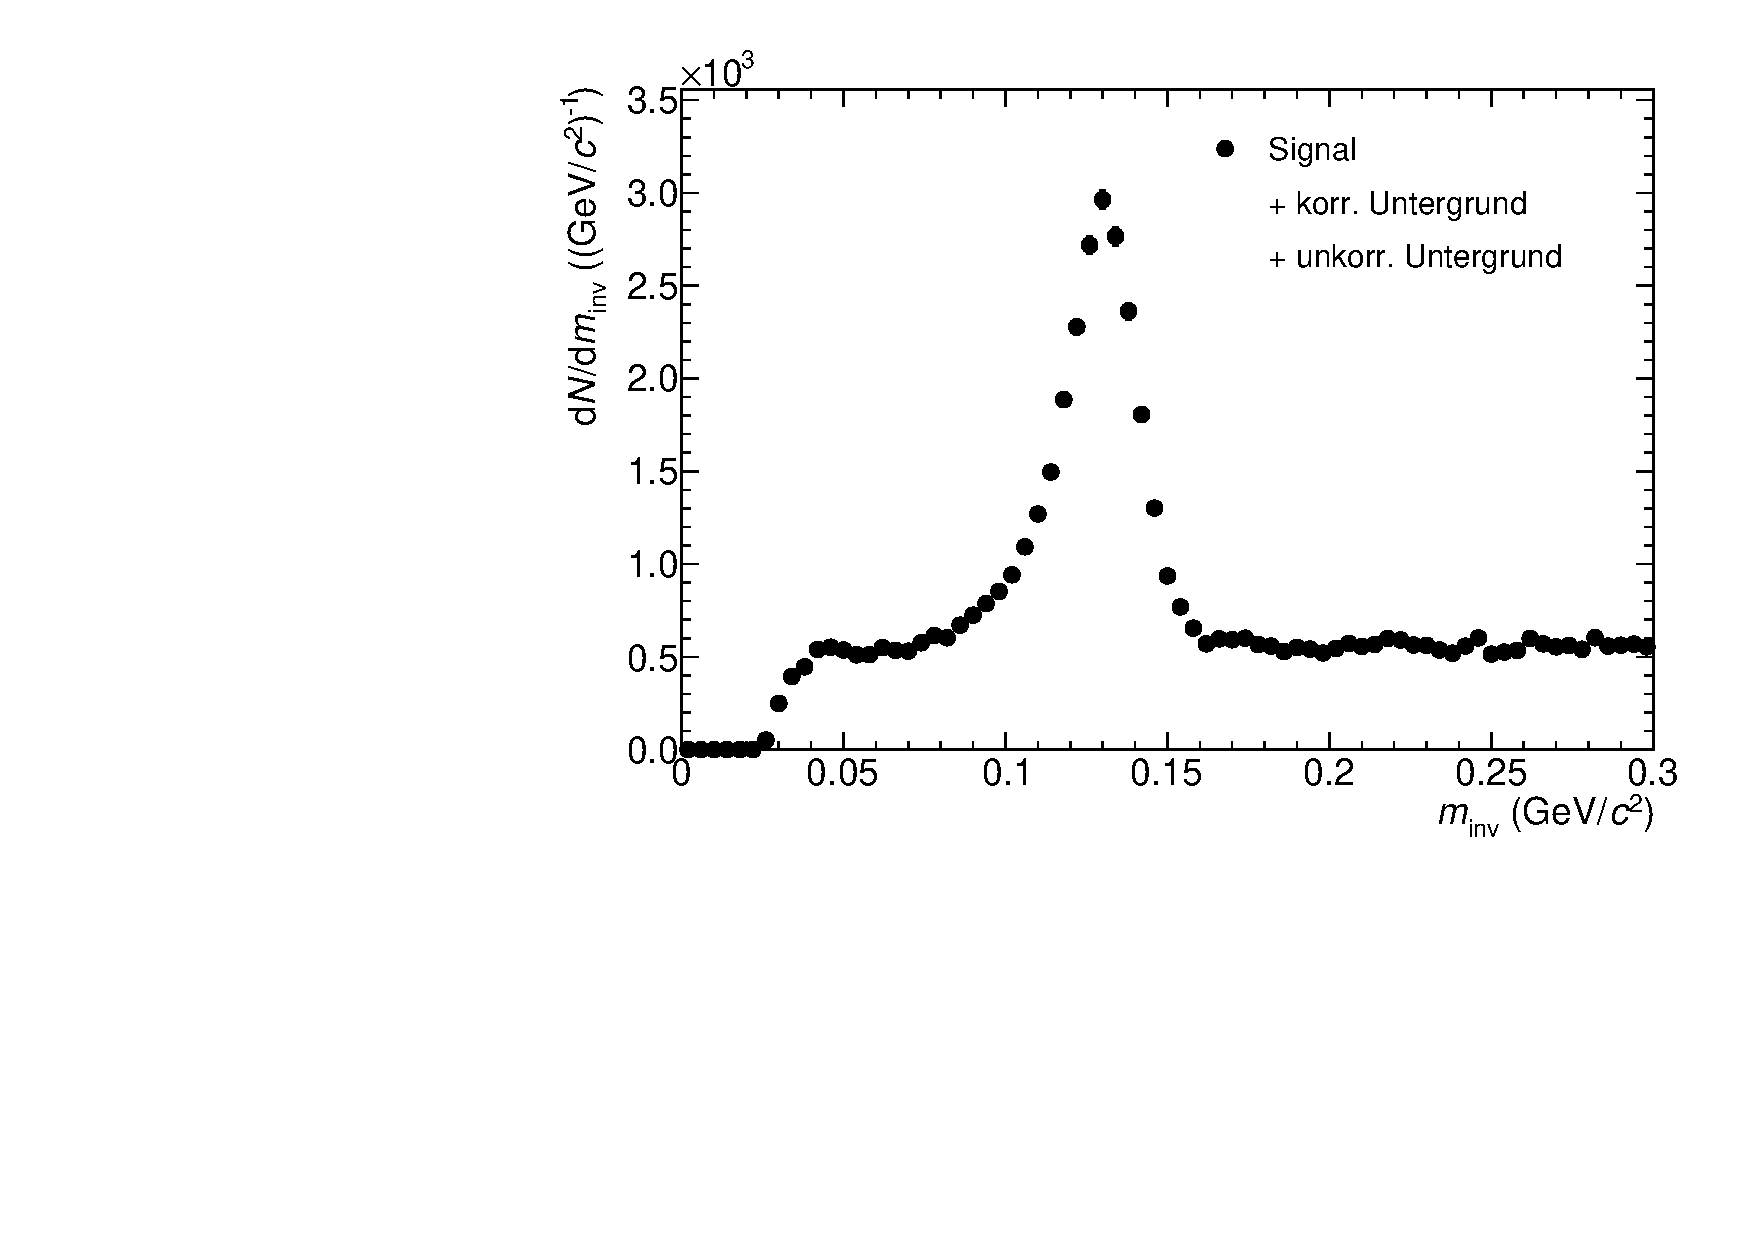
\includegraphics[width=.75\linewidth]{hSignalPlusBkg.pdf}
\caption{Projektion von Abbildung \ref{figInvMassPt_a} im $p_{\text{T}}$-Intervall $(3,2 - 3,4) (\text{GeV/}c)$. Es ist ein deutlicher Peak um $m_{\pi^{0}} \approx 0,135\text{ GeV/}c^{2}$ zu erkennen, aber auch Untergrund, da das Signal zu h{\"o}heren Massen gau{\ss}f{\"o}rmig abklingen sollte. Bei $m_{\text{inv}} < m_{\pi^{0}}$ kann Signal vorliegen, das aus konvertierten Photonen besteht, weshalb eine Aussage {\"u}ber die Form, bzw. den Untergrund dort schwer m{\"o}glich ist.}
\label{figSignalPlusBkg}
\end{figure}
\newline
Abbildung \ref{figSignalPlusBkg} zeigt eine Verteilung der invariante Massen in einem $p_{\text{T}}$-Intervall von $(3,2 - 3,4)(\text{GeV}/c)$.
Die zuvor beschriebene Anh\"aufung von Datenpunkten in Abbildung \ref{figInvMassPt_a} zeigt sich auch hier deutlich und wird im Folgenden als Peak bezeichnet.
Der Peak besteht wie oben erw\"ahnt hauts\"achlich aus richtig rekombinierten $\pi^{0}$.
Neben dem Signal besteht die Verteilung in Abbildung \ref{figSignalPlusBkg} noch aus sogenanntem Untergrund, der in zwei Teile unterteilt wird, den kombinatorischen oder auch unkorrelierten Untergrund und dem korrelierten Untergrund.
Dem korrelierten Untergrund hingegen liegen paarweise Kombinationen von Photonenkandidaten zugrunde, zwischen denen eine Korrelation besteht.
Das hei{\ss}t, dass die Photonenkandidatenpaare nicht aus dem Zerfall eines $\pi^{0}$ stammen, aber \"uber einen anderen Zerfall zusammenh\"angen.
Durch die paarweise Kombination unkorrelierter Photonenkandidaten, also solcher, die nicht aus einer Zerfallsk\"atte stammen, entsteht der unkorrelierte Untergrund.
\newline
Im folgenden Abschnitt wird eine Methode zur Absch\"atzung des unkorrelierten Untergrunds vorgestellt. 